\section{Nombre: Xochitónal}  \label{per:xochitonal}

\subsection{Descripción:}
Iguana gigante de color rojo grisáceo y ojos naranjas. Porta una armadura de huesos que protege su espina dorsal, y su rostro.
\\
\par
Xochitonal normalmente es de actitud calmada y carácter amable. Disfruta de nadar y evita en la medida de lo posible salir del agua, ya que es el lugar en donde se siente más seguro.  
\subsection{Status:}
	\begin{itemize}
		\item Personaje no jugable.
		\item Enemigo jefe.
	\end{itemize}
\subsection{Imagen}
Ver figura \ref{fig:XochitonalDiseno}
\begin{figure}
				\centering
				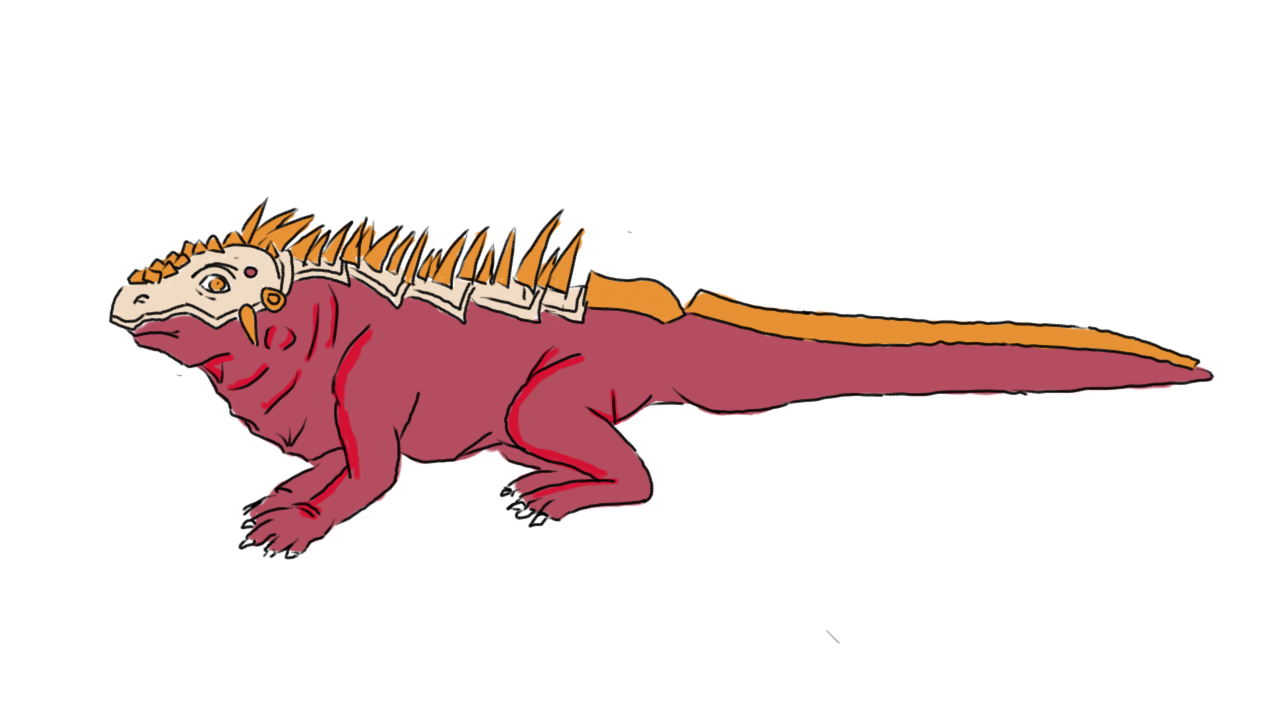
\includegraphics[height=0.3 \textheight]{Imagenes/Xochitonal}
				\caption{Concepto de diseño de Xochitonal.}
				\label{fig:XochitonalDiseno}
\end{figure}
\subsection{Concepto:}
\begin{itemize}
	\item \textbf{Historia antes del juego:}
	Xochitónal es el único guardián del Mictlán que no es un Dios. Creado por Mictlantecuhtli durante la era posterior al Quinto Sol. Xochitónal tiene como deber proteger la entrada al Mictlán, motivo por el que patruya el rio Apanohuacalhuia y debora las almas de todos aquellos que no sean dignos de la ayuda de un Xoloitzcuintle o que por diversos motivos no lograron pasar.
	\item \textbf{Historia durante el juego:}
	Xochitónal es el primer jefe a derrotar por lo que su rol no tiene mucho peso sobre la historia.
	\item \textbf{Relaciones:}
	\begin{itemize}
		\item \textbf{Mictlantecuhtli:} Es su creador. Xochitónal guarda un profundo respeto por él y procura a odecerlo en la medida que sus habilidades se lo permitan. Su lealtad hacia él es tanta que Xochitónal esta dispuesto a morir por su creador (ver aparatado \ref{per:mictlantecutli}). 
		\item \textbf{Mictecacíhuatl:} Como esposa de su creador. Xochitónal tiene una relación de absoluto respeto hacia la reina del Mictlán (ver aparatado \ref{per:mictecacihuatl}). 
		\item \textbf{Xólotl:} Dado que fue creado después del quinto sol, nuca pudo convivir con Xólotl por lo que su opinion hacia él se basa totalmente en lo poco que ha escuchado de los demás guardianes del inframundo (ver aparatado \ref{per:xolotl}).
	\end{itemize}			  
\end{itemize} 
\subsection{Encuentro:}
\begin{itemize}
	\item Su primera aparición es en la cinemática 5 (ver aparatado \ref{Cin:Cinematica05}). 
	\item El jugador se enfrenta a él como jefe del segundo nivel del juego (ver aparatado \ref{Nivel:Niv02}).
\end{itemize}
\subsection{Habilidades:}
Al ser el guardián del río  Apanohuacalhuia, las habilidades de Xochitónal son sobre el control del agua:
\begin{itemize}
	\item Zambullida (ver aparatado \ref{hab.zambullida}).  
	\item Burbujas (ver aparatado \ref{hab.burbujas}).
\end{itemize}
\subsection{Armas:}
Sin armas.
\subsection{Ítems:}
Sin ítems.
\subsection{Bloques de animación}
	\begin{itemize}
		\item Animación emerge del agua.
		\item Animación se sumerge en el agua.
		\item Animación Dispara burbujas.  
		\item Animación recibir daño.
	\end{itemize}